\documentclass[12pt,a4paper,oneside]{report}
% nagyon sok kép esetén meggyorsítható a fordítás a draft móddal
% \documentclass[12pt,a4paper,oneside,draft]{report}
% ekkor a képek nem renderelődnek ki, csak placeholder lesz mérethelyesen
\usepackage[utf8]{inputenc} % mindenképp maradjon az utf-8 kódolás
\usepackage[magyar]{babel}
\usepackage[T1]{fontenc}
\usepackage{float}
\usepackage{wrapfig}
\usepackage{subcaption}
\usepackage[export]{adjustbox}
\usepackage{amsmath}
\usepackage{amsfonts}
\usepackage{amssymb}
\usepackage{graphics} % grafikus elemek, képek berakásához
\usepackage{epsfig} % eps importáláshoz
\usepackage{listings}
\usepackage{sectsty}
\usepackage{enumerate}
\usepackage{lastpage}
\usepackage{setspace}
\usepackage{hyperref} % PDF hivatkozásokhoz kell
% \usepackage[hang]{caption}
\usepackage{caption}
\usepackage{titling} % a title, author parancsok szabad használatához

% a TikZ rajzoló modul, és a kapcsolási rajz készítő modul, ha kell
%\usepackage{tikz}
%\usepackage{circuitikz}

% az A4 oldal margóinak és méreteinek beállítása
\usepackage[left=25mm,right=25mm,top=20mm,bottom=25mm]{geometry}\pagestyle{plain}

% A sorköz távolság beállítása
% egyszeres sorköz
\singlespacing
% 1,5 sorköz
% \onehalfspacing

% A hivatkozások, és linkek átállítása alapértelmezett színre, fekete-fehér nyomtatáshoz optimalizálva
\hypersetup
{
  	colorlinks,
  	citecolor=black,
 	linkcolor=black,
  	urlcolor=black
}

% --------- A hallgató által kitöltendő rész! --------- %

% a dolgozat típusa
\title{Önálló laboratórium beszámoló} 

% a dolgozat szerzője
\author{Bálint Éliás}

% a dolgozat típusát adjuk meg tárgyesetben, kisbetűvel (pl.: diplomatervet, szakdolgozatot, témalabor beszámolót stb.)
\newcommand{\dokumentumtipus}{önálló labor beszámolót} 

% a dolgozat témája
\newcommand{\dokumentumcim}{Szinkronizációs eljárások vizsgálata 5G OFDMA rendszerekben IEEE specifikációk alapján}

% --------- A hallgató által kitöltendő rész! --------- %

\begin{document}
\begin{titlepage}

\begin{figure}
\centering

\includegraphics[width=100mm,keepaspectratio]{bme.pdf}
\end{figure}

\centering
\textbf{Budapesti Műszaki és Gazdaságtudományi Egyetem}\\
\textbf{Villamosmérnöki és Informatikai Kar}\\
\textbf{Szélessávú Hírközlés és Villamosságtan Tanszék}\\
\vspace{5mm}

\includegraphics[width=40mm,keepaspectratio]{hvt_logo_only_fixed_vector_inverted.png}  \\
\vspace{40mm}
\Huge
\dokumentumcim\\
\vspace{50mm}
\Large
\thetitle \\
\vspace{12mm}
\Large
\textbf{\theauthor}\\
\vspace{12mm}
\the\year


\end{titlepage}
% \newpage
\hspace{10mm}
\begin{center}
\large
\textbf{HALLGATÓI NYILATKOZAT}
\end{center}
\hspace{10mm}

Alulírott \theauthor, szigorló hallgató kijelentem, hogy ezt a \dokumentumtipus \ meg nem engedett segítség nélkül, saját magam készítettem, csak a megadott forrásokat (szakirodalom, eszközök stb.) használtam fel. Minden olyan részt, melyet szó szerint, vagy azonos értelemben, de átfogalmazva más forrásból átvettem, egyértelműen, a forrás megadásával megjelöltem.

Hozzájárulok, hogy a jelen munkám alapadatait (szerző(k), cím, angol és magyar nyelvű tartalmi kivonat, készítés éve, konzulens(ek) neve) a BME VIK nyilvánosan hozzáférhető elektronikus formában, a munka teljes szövegét pedig az egyetem belső hálózatán keresztül (vagy autentikált felhasználók számára) közzétegye. Kijelentem, hogy a benyújtott munka és annak elektronikus verziója megegyezik. Dékáni engedéllyel titkosított diplomatervek esetén a dolgozat szövege csak 3 év eltelte után válik hozzáférhetővé.

\hspace{10mm}

Budapest, \today

\begin{flushright}
\theauthor
\end{flushright}
% Ide kell include-olni, vagy befűzni a feladatkiírást, ha van
\tableofcontents
% \chapter*{Kivonat}

Jelen dokumentum egy diplomaterv sablon, amely formai keretet ad a BME Villamosmérnöki és Informatikai Karán végző hallgatók által elkészítendő szakdolgozatnak, és diplomatervnek. A sablon használata opcionális. Ez a sablon \LaTeX \  alapú, a TeXLive TeX 
implementációval és a PDF-LaTeX fordítóval működőképes.

% \chapter*{Abstract}

This document is a \LaTeX -based template for the BSc/MSc thesis of students at the Electrical Engineering and Informatics Faculty of Budapest University of Technology and Economics. The usage of this template is optional. It has been tested with the TeXLive TEX implementation, and it requires the PDF-LaTeX compiler.
\chapter{Bevezetés}

\section{Előző féléves munkám}

A Budapesti Műszaki és Gazdaságtudományi Egyetem Villamosmérnöki és Informatikai karán a villamosmérnök alapszak 5. félévében Témalaboratórium tantárgyat hirdetnek.
Ez a tantárgy egy olyan projekttárgy, amely a hallgatók számára lehetővé teszi, hogy valamilyen területen elmélyedjenek, és közösen dolgozzanak egy témavezetővel, ezzel tapasztalatot nyújtva számukra, a későbbi Önálló laboratórium és Szakdolgozat készítés tárgyakhoz.

Én az 5. félévemben a Témalaboratórium keretei között Dr. Horváth Bálint Péter témavezetésével folytattam egyéni munkát, amely során egy OFDM (Orthogonal Frequency Division Multiplexing - Ortogonális Frekvenciaosztásos Nyalábolás) rendszert modelleztem. A munka során Python nyelvben készítettem el egy digitális jelátvitel rendszer modelljét, amelyben az adót, a vevőt, és köztük az átviteli csatorna volt a 3 legfőbb elem. Munkám során azt vizsgáltam, hogy miképp tud egy ilyen OFDM rendszer védekezni a többutas terjedés problémái ellen, milyen lehetőségek vannak a vett jel kompenzálására, vagy az átvitel minőségének mérésére.

Az eredmények részletes tárgyalása nem része ennek a dolgozatnak, de az eredményeket is és a tanultakat is felhasználtam a féléves munkámban.

\section{OFDM és OFDMA}

Az OFDM és az OFDMA (Orthogonal Frequency Division Multiple Access) rendszerek között egy apró különbség van. Míg egy OFDM rendszerben egy adó és egy vevő közötti kommunikáció valósul meg több vivőfrekvencián, addig az OFDMA rendszerben a kommunikáció egy vagy több adó és egy vagy több vevő között valósul meg. Ez számomra nem volt evidens, a tanulmányaim során eddig a kettőt összemosták.

Az OFDM előnyeit könnyedén kihasználhatjuk többszörös hozzáférési rendszerekben is.
Így nevezzük azokat a rendszereket, amelyekben egyszerre párhuzamosan több jelátvitel valósul meg.
Ezt megtehetjük a frekvenciatartománybeli szétválasztással, lásd a GSM uplink és downlink kapcsolat, ahol két teljesen elkülönülő frekvenciatartományt vesz igénybe a kétfajta átvitel. 
Ugyanez a hatás elérhető, ha az átviteli médiumot valamilyen időosztásban osztjuk fel a felhasználók között. 
Van olyan módszer is, amellyel időben és frekvenciában is egyszerre oldhatjuk meg az ütközéseket, ha megfelelően kódoljuk az átvinni kívánt jelet.

\section{OFDMA kihívásai}

xdxd

\section{Munkám}
% \include{attekintes}
\chapter{5G architektúra}

Az 5G architektúra az ötödik generációs mobilhálózati technológia alapját képezi, amely jelentős előrelépést jelent a korábbi generációkhoz képest, mind a sebesség, mind a kapacitás és a megbízhatóság tekintetében.
Az 5G rendszer alapvetően három fő komponensből áll:

\begin{itemize}
    \item Felhasználói Berendezések (User Equipment, UE): Ezek a végfelhasználói eszközök, mint például okostelefonok, táblagépek, és más, 5G-képes eszközök, amelyek csatlakoznak a hálózathoz.
    \item Rádió Hozzáférési Hálózat (Radio Access Network, RAN): Ez a hálózati komponens biztosítja a vezeték nélküli kapcsolatot a felhasználói berendezések és a központi hálózat között.
    Az 5G RAN magába foglalja a következő elemeket:
    \begin{itemize}
        \item gNodeB (gNB): Ez az új bázisállomás, amely a rádió interfészt biztosítja a felhasználói eszközök számára.
        \item Massive MIMO és Beamforming technológiák, amelyek javítják a hálózat kapacitását és hatékonyságát.
    \end{itemize}
    \item Core Hálózat (Core Network, CN): Az 5G core hálózat a hálózat központi részét alkotja, amely az adatforgalom kezelését, a felhasználói autentikációt, és a hálózati szolgáltatások biztosítását végzi.
    Az 5G core hálózat a következő komponensekből áll:
    \begin{itemize}
        \item User Plane Function (UPF): Az adatforgalom útvonalát kezeli.
        \item Access and Mobility Management Function (AMF): A felhasználói eszközök mobilitását és hálózathoz való hozzáférését kezeli.
        \item Session Management Function (SMF): A felhasználói adatszolgáltatásokat és azok konfigurációját kezeli.
    \end{itemize}
\end{itemize}

Az 5G architektúra különlegessége, hogy támogatja a virtualizációt és a hálózati szeletelést (network slicing), amely lehetővé teszi, hogy különböző szolgáltatások és alkalmazások eltérő hálózati igényekkel különálló szeleteket kapjanak ugyanazon fizikai hálózaton belül.
Ez növeli a hálózat rugalmasságát és hatékonyságát, biztosítva a különféle felhasználói esetek, mint például az autonóm járművek, az IoT eszközök és a nagy felbontású videostreaming igényeinek kielégítését.

\section{Rádiós Hozzáférési Hálózat}

Az 5G hálózatok fizikai rétegének specifikációja a 3rd Generation Partnership Project (3GPP) nevű szervezet nevéhez kötődik.
A szervezet felelős a mobil kommunikációs hálózatok egységesítéséért, fejlesztéséért és működtetéséért.
Az új generációs ??????????

\begin{figure}[h]
    \centering
    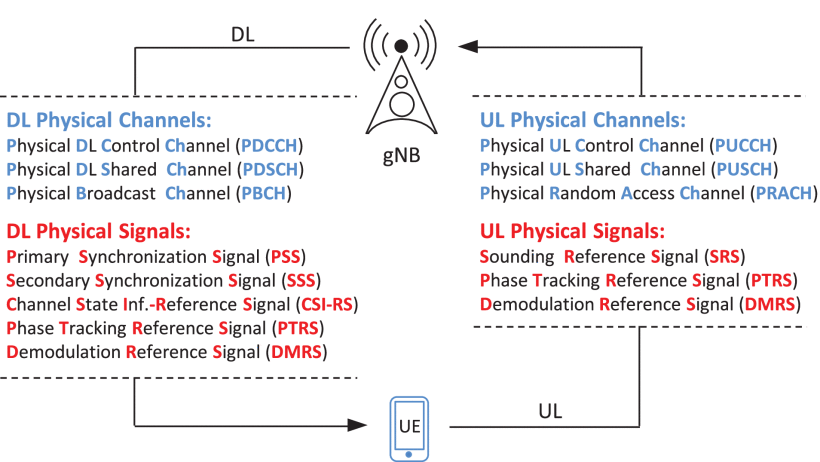
\includegraphics[width=0.6\textwidth]{jelek.png}
    \caption{Az 5G NR fizikai csatornái és jelei}
    \label{fig:jelek}
\end{figure}

\subsection{5G NR keretstruktúra}

% \begin{wrapfigure}{r}{0.38\textwidth}
%     \begin{center}
%         % \setlength{\fboxrule}{1pt}%
%         % \fboxrule=1mm
%         \fboxsep=1mm
%         \fbox{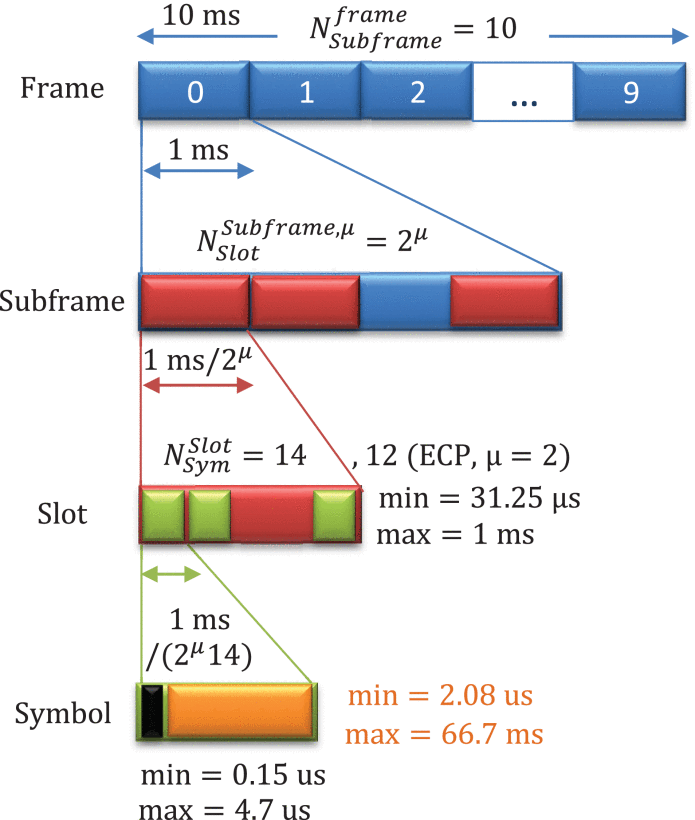
\includegraphics[width=0.36\textwidth]{slot.png}}%
%     %   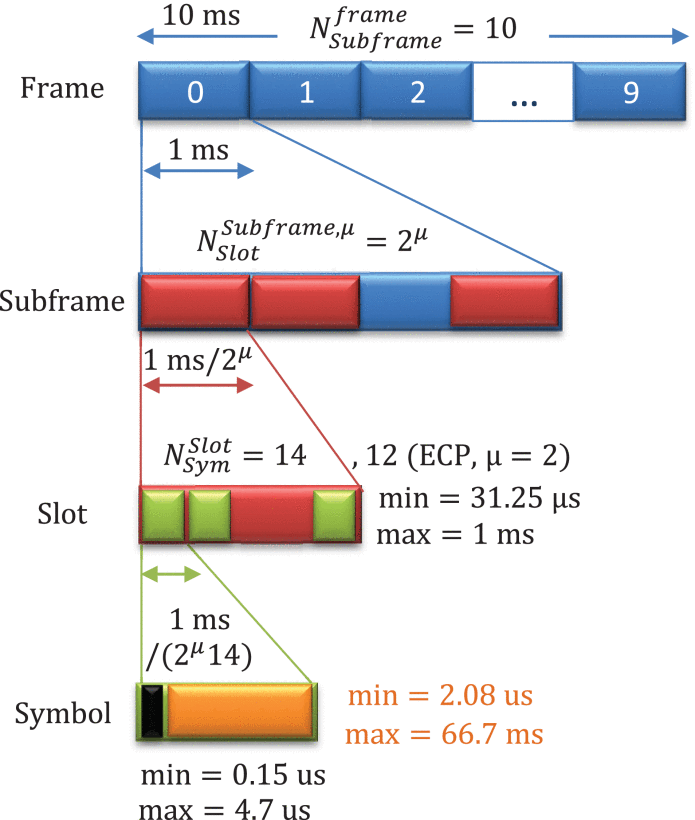
\includegraphics[width=0.38\textwidth, frame]{slot.png}
%     \end{center}
%     \caption{Birds}
%   \end{wrapfigure}

az 5G NR keretstruktúrája $N_{Subframe}^{frame}=10$ subframe-ből áll, amely közül mindegyik 1 ms idejű.
Különbség az LTE hálózatokhoz képest, hogy egy 5G NR subframe változó számú slotot tartalmaz, amelyet az alkalmazott numerológia határoz meg ($\mu$) a következő módon: $N_{Slot}^{Subframe,\mu}= 2 ^\mu$.
Ennek megfelelően egy slot időtartama $ t = \dfrac{1 \text{ ms}}{2^\mu}$.
Végezetül minden slot tartalmaz 12/14 OFDM szimbólumot attól függően, hogy normál/kiterjesztett ciklikus előtagot alkalmaz a rendszer.
Ebből következik, hogy egy OFDM szimbólum időtartama $ t = \dfrac{1 \text{ ms}}{2^\mu 12}$ vagy $ t = \dfrac{1 \text{ ms}}{2^\mu 14}$.

\begin{figure}[h!]
    \centering
    \fboxsep=1mm
    \fbox{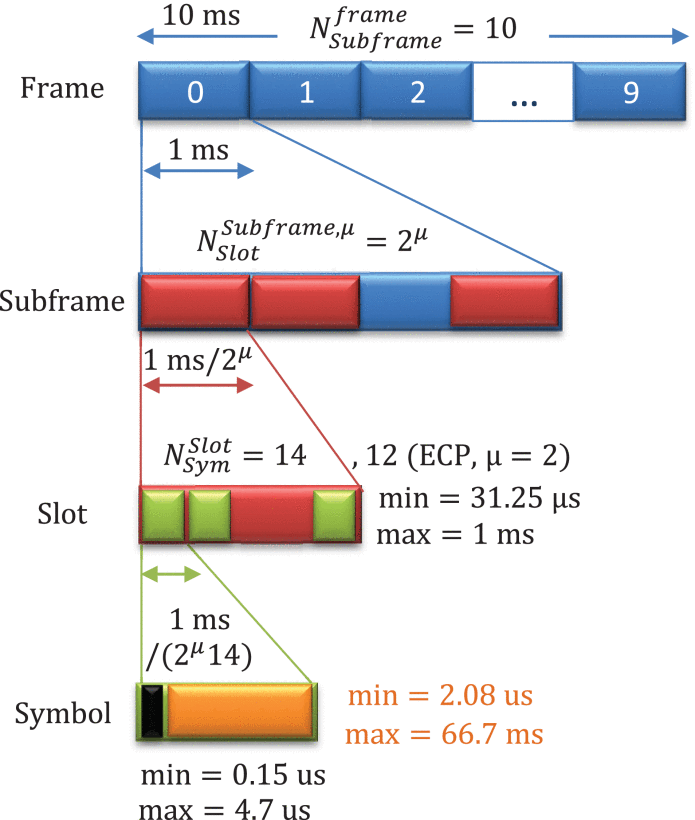
\includegraphics[width=0.4\textwidth]{slot.png}}
    % TODO: MELLÉ A KÉPLETEK
    \caption{Az 5G NR keretstruktúrája}
    \label{fig:slot}
\end{figure}



Mivel a rendszer OFDMA alapú, ezért frekvenciatartományban ún. Resource Blockokat (RB) definiál a 3GPP szabvány, mégpedig egy RB 12 egymást követő alvivőt foglal magába.
Legyen $\Delta f$ az alvivőtávolság: az 5G NR rendszerben $\Delta f$ flexibilis, és az alkalmazott numerológiától függ. $\Delta f = 15 \text{ [kHz] } 2^\mu$.


\section{Kiindulási pont}

Tekintsük az alapállapotot. Ilyenkor minden kapcsolat stabil.
Minden felhasználói készülék (User Equipment - UE) tudja, hogy milyen frekvenciacsoportban kommunikál melyik alállomással (bázisállomás).
A készülékek nem mozognakés nem történik handover.
Ebben az állapotban kapcsolunk be egy telefont.
A bekapcsoló telefon értelemszerűen elkezdi keresni a hálózatot, hogy létrejöhessen a kapcsolat, amelynek feltétele, hogy a telefon elvégezze a szinkronizációs lépéseket, és dekódolja, hogy melyik frekvenciákon kommunikálhat az alállomással.
\chapter{Szinkronizáció 5G NR rendszerekben}

\section{Szinkronizációs jelek}

\subsection{Primary Synchronization Signal}

5G NR hálózatokban az elsődleges szinkronizáló jel a cella ID szektor ($N_{ID}^{(2)}$) dekódolására alkalmas az UE számára.
A jel segítségével az UE meghatározhatja a mintavételezés frekvenciájéának hibáját, és helyreállíthatja a későbbi jeleket vevőoldalon.

Az 5G-NR PSS három különböző 127 szimbólumú m-szekvenciából áll amelyek 127 alvivőt használnak fel. A 3 lehetséges m-sorozat a következőféleképp van definiálva:

\begin{align}
    d_{PSS}(n) &= 1-2x(m)
\end{align}

ahol

\begin{align}
    m &= [n+43N_{ID}^{(2)}] \text{ mod } 127\\
    x(i + 7) &= [x(i + 4) + x(i)] \text{ mod } 2
\end{align}

illetve

\begin{align}
    [x(6)\; x(5)\; x(4)\; x(3) \;x(2)\; x(1) \;x(0) ] &= [1 \;1\; 1\; 0\; 1\; 1\; 0]
\end{align}

\subsection{Secondary Synchronization Signal}

5G NR hálózatokban az másodlagos szinkronizáló jel a cella ID csoport ($N_{ID}^{(1)}$) dekódolására alkalmas az UE számára.
Az SSS-t követően a UE oldalon kiszámítható a pontos Cella ID a következő módon: $ N_{ID}^{cella} = 3 N_{ID}^{(1)} + N_{ID}^{(2)}$.

Az 5G-NR SSS 355 különböző 127 szimbólumú gold-szekvenciából áll amelyek 127 alvivőt használnak fel. A 355 lehetséges gold-sorozat a következőféleképp van definiálva:

\begin{align}
    d_{SSS}(n) &= [1 - 2 x_0 ([n + m_0] \text{ mod } 127)][1 - 2 x_1 ([n + m_2] \text{ mod } 127)]
\end{align}

ahol

\begin{align}
    m_0 &= 15[\frac{N_{ID}^{(1)}}{112}] + 5 N_{ID}^{(2)}\\
    m_1 &= N_{ID}^{(1)}  \text{ mod } 112, 0 \leq n < 127\\
    x_0 (i + 7) &= [x_0 (i + 4) + x_0 (i)] \text{ mod } 2\\
    x_1 (i + 7) &= [x_1 (i + 4) + x_1 (i)] \text{ mod } 2\\
    [x_0(6) \; &x_0(5) \;  x_0(4) \;  x_0(3) \;  x_0(2) \;  x_0(1)  \; x_0(0) ]\\
     &= [0 \;  0 \;  0 \;  0  \; 0  \; 0 \;  1] 
\end{align}

illetve

\begin{align}
    [x_1(6) \;x_1(5)\; x_1(4)\; x_1(3)\; x_1(2)\; x_1(1)\; x_1(0) ] &= [0\; 0\; 0\; 0\; 0\; 0\; 1]
\end{align}

\section{Szinkronizáció PSS-sel}

A Témalaboratórium tárgy keretei között egy OFDM rendszer előnyös tulajdonságaival foglalkoztam egy egyvivős modulációs rendszerrel szemben.
Az OFDM egyik előnye, hogy úgynevezett pilot-vivők (segédvivők) segítségével a vevőoldalon hatékonyan tudjuk becsülni a csatorna átviteli karakterisztikáját, amellyel a vett jelet kompenzálni tudjuk.
Másik előnye az OFDM-nek, hogy ciklikus előtagot alkalmaz, vagyis minden szimbólum végét az elejére másolja a védőidő helyére, ez a szimbólumváltás tranziensét hivatott csökkenteni, azonban az OFDM szimbólumok kezdetét is megtalálhatjuk, ha a vett jelben ismétlődéseket keresünk.

Az 5G NR rendszerben a vevő szinkronizációja a megadott szinkronizációs jelek (PSS és SSS) dekódolásával történik.
A felhasználói készülék ezeket a jeleket felhasználva képes a hálózatra kapcsolódni.

\subsection{A vett jelek matematikai leírása}

Legyen $ r(n) $ egy ideálisan vett és mintavételezett jel vevőoldalon.

\begin{align}
    r(n) &= s(n) \ast h(n) + w(n)\\
    r_{\epsilon} (n) &= [s(n) \ast h(n) + w(n)] exp(\frac{j 2 \pi n }{N_{FFT}} \epsilon) \label{eq:frekhiba}
\end{align}

$\epsilon$ a normalizált frekvenciahiba, amelyet egész és tört komponensekre tudunk bontani.

\subsection{Szinkronizációs algoritmus}

Mivel $\epsilon$ egészrésze valójában egy egésszel való eltolást okoz a vett jel időtartoményi reprezentációjában, ezért azt könnyen figyelmen hagyhatjuk.
Legyen $ \hat{\theta} $ a PSS-hez tartozó időpont becslője, $ \hat{i} $ pedig cella ID szektor becslője ($ \hat{i} \in {0, 1, 2} $).

Ezt a két ismeretlent a következő módon becsülhetjük:

\begin{equation}
    (\hat{\theta},  \hat{i}) = arg max (C(\theta, i))
\end{equation}

Ahol $ C(\theta, i) $ a keresztkorrelációt jelöli, mégpedig:

% \begin{equation}
%     C(\theta, i) = \frac{ \vert \sum_{k=0}^{N_{FFT} - 1} r(\theta + k) p_i^\ast (k) \vert }{\sum_{k=0}^{N_{FFT} - 1} \vert r(\theta + k) \vert^2 }
% \end{equation}

\begin{equation}
    C(\theta ,i)=\frac { \left |{\sum \limits _{k=0}^{N_{_{\text {FFT}}}-1}{r(\theta +k) p_{i}^{*}(k)}}\right |}{\sum \limits _{k=0}^{N_{_{\text {FFT}}}-1}{ \left |{r(\theta +k)}\right |^{2}}}
\end{equation} 

Ahol $r(\theta + k)$ a vett késő jelet jelöli, $ p_i (k) $ az $i$-edik cella ID szektor PSS jelének időtartománybeli alakja, $N_{FFT}$ pedig a CP nélküli mintaszám.
Ebben az esetben A frekvencia törtrészére a következő becslést adhatjuk:

% \begin{align}
%     \hat {\epsilon }_{_{F}}=&\frac {1}{\pi } \angle \Bigg (\left[{ \sum \limits _{k=0}^{N_{_{\text {FFT}}}/2-1}{r(\hat {\theta }+k) p_{\hat {i}}^{*}(k)}}\right]^{^{*}} \\&\qquad \times \left[{ \sum \limits _{k=N_{_{\text {FFT}}}/2}^{N_{_{\text {FFT}}}-1}{r(\hat {\theta }+k) p_{\hat {i}}^{*}(k)}}\right] \Bigg)
% \end{align} 

\begin{equation}
    \hat {\epsilon }_{_{F}}=\frac {1}{\pi } \angle \Bigg (\left[{ \sum \limits _{k=0}^{N_{_{\text {FFT}}}/2-1}{r(\hat {\theta }+k) p_{\hat {i}}^{*}(k)}}\right]^{^{*}}  \times \left[{ \sum \limits _{k=N_{_{\text {FFT}}}/2}^{N_{_{\text {FFT}}}-1}{r(\hat {\theta }+k) p_{\hat {i}}^{*}(k)}}\right] \Bigg) \label{eq:hibabecsles}
\end{equation} 

\subsection{Magyarázat}

A vevőoldalon (UE) az eszközben található oszcillátor hibája nagyban befolyásolja a vétel minőségét, és mivel GHz feletti tartományban mozgunk, ezért a frekvenciahiba a jelet elrontja.
Ezt a hibát reprezentálja a \ref{eq:frekhiba} képletben szereplő exponenciális tag.
Gyakorlatilag a mintavételi frekvencia hibája egy folytonos fázishibaként fogható fel a jelben, és pont ez teszi lehetővé, hogy a hibát becsüljük.

Mivel a szinkronizációs jelek ismertek, ezért a vevőoldalon a vett jelet keresztkorrelálva az ismert PSS szekvenciákkal megtalálhatjuk a PSS szimbólum kezdetét.
Mivel tudjuk, hogy melyik PSS szimbólum keresztkorrelációja adja a legnagyobb korrelációs együtthatót, így a Cella ID szektort is megállapíthatjuk.

Végezetül már csak arra van szükségünk, hogy a vett PSS szimbólum és az eredeti PSS szimbólum különbségéből a frekvenciahibát megállapítsuk, amelyet szintén a keresztkorreláció eredményének fázisa mutat meg (lásd \ref{eq:hibabecsles} képlet).
A \ref{eq:hibabecsles} képlet alapja, hogy a PSS szimbólum első felének korrelációs együtthatójának fázisát és a második felének korrelációs  együtthatójának fázisából megkaphatjuk, hogy a PSS szimbólum átvitele alatt mennyit változott a fáziskülönbség, amelyből a frekvenciahibát kiszámíthatjuk (Fontos, hogy az eredmény a normalizált frekvenciahibát adja meg, tehát független az alkalmazott 5G numerológiától).

\section{SSS dekódolása}

Miután megmértük a helyi frekvenciahibát, és abból visszaállítottuk az eredeti jelet, a másodlagos szinkronizációs jelet kell dekódolni.
Az összes lehetséges SSS definiálva van a vevő számára, és a jel kezdete is ismert, ha a PSS helyét már ismerjük.

A dekódolás a PSS-hez hasonlóan keresztkorreláció számítással történik, azonban ennek magasabb erőforrás igénye van, hiszen nagyságrendekkel több lehetséges SSS jellel kell korreláltatni a vett jelet, hogy a valódit megtaláljuk.
\chapter{Szimulációs eredmények}

\section{Szimulációs környezet}

A szimulációkat Python környezetben végeztem el, ahol a számítások jelentős részét a numpy könyvtár segítségével implementáltam, az eredmények értékeléséhez pedig a matplotlib könyvtárat használtam fel.
A szimuláció során egy Cella ID-ra vonatkoztatva végeztem el a méréseket, méghozzá a 120-as sorszámúra.
256 alvivővel végeztem a szimulációkat, így az $N_{FFT} = 256$.

A szimulált szinkronizációs jeleket a szabvány szerint generáltam, az egyetlen különbség az volt, hogy közöttük nem hagytam védőidőt, a PSS-t azonnal az SSS követi.
A két jel előtt és után védőidőt hagytam, itt csak zaj van a jelben.

\begin{figure}[h]
    \centering
    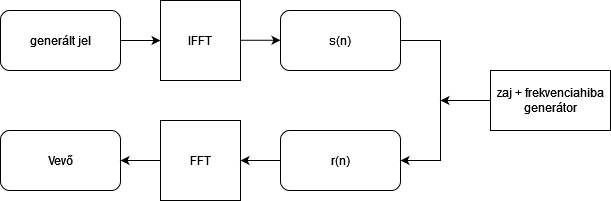
\includegraphics[keepaspectratio, width = 0.8\textwidth]{onlab.drawio.png}
    \caption{A szimulált rendszer blokkvázlata}
\end{figure}

A jelfeldolgozási és szinkronizációs feladatokat a vevő végzi el.
A szimulációt -45 dB és 5 dB között változó jel-zaj viszonnyal végeztem el, és mindegyik esetben 1000-szer szimuláltam egy szinkronizációs burstöt.

\section{PSS megkeresése}

\section{SSS dekódolása}

\section{Hibabecslés}




% \chapter*{Köszönetnyilvánítás}
Ide kerül az opcionális köszönetnyilvánítás, amelyben érdemes megemlíteni a konzulenst, illetve mindazokat, akik a dolgozat létrejöttében segítettek a szerzőnek. 
\begin{thebibliography}{4}

\bibitem{hvthonlap} \url{http://hvt.bme.hu}

\bibitem{radiotechnika} Rádiótechnika évkönyve 2007, 172. oldaltól

\bibitem{diploma} Dudás Levente, \emph{Digitális nyalábformálású antenna (DBF)} diplomaterv, BME SzHVT, 2007

\bibitem{kicad} \url{http://kicad-pcb.org/}

\end{thebibliography}


% \listoffigures
% \listoftables
\chapter*{Függelék}

A függelék az a fejezet, amely nem képezi szerves részét magának a dolgozatnak (nem növeli az oldalszámot), csak a megértést segíti, illetve a plusz ábrákat, pl. kapcsolási rajzokat, NYÁK terveket, program forráskódokat tartalmazza, de természetesen lehet hivatkozni rá (és sok esetben kell is). \label{fugg}

Jelen dokumentumot, nemcsak pdf, hanem \LaTeX \  forráskód szinten is közzéteszem, abból a megfontolásból, hogy lehetőség szerint legyen egységes a beadott beszámolók és jegyzőkönyvek formátuma és kinézete.

Jelen dokumentum forráskódja példákat tartalmaz a szövegek, képek, táblázatok, számozott és számozatlan felsorolások szerkesztésére, tagolására, formátumára vonatkozóan beleértve a matematika kifejezések forráskód szintű kezelését is.

A LaTeX letölthető többféle operációs rendszerre innen: 
\\
\url{https://www.latex-project.org/get/}

Ha valakinek magyar nyelvű szótárra van szüksége, akkor használhatja jelen dokumentum mappájában levő állományt is: a fordítóban kell beállítani a nyelvi beállításoknál.

% végső fordításnál kapcsold ki a draft módot !!

\end{document}